\chapter{Desarrollo}

En este capítulo se describe de manera detallada el desarrollo del clasificador de tubérculos siguiendo la metodología descrita en el capítulo 3.
\noindent
\section{Comprensión de datos}

\noindent
\textbf{Recolección de datos iniciales.}\\

Los datos empleados para realizar la clasificación fueron previamente recolectados por Bernal (2017). En un estudio que se realizó en el Centro agropecuario Marengo de la Universidad Nacional de Colombia, en el departamento de Cundinamarca (74°12'58.51 W; 4°40'52.92 N), el cual tiene una altitud de 2516 msnm, temperatura media de $14^\circ$C  en un rango de $12^\circ$C  a $18^\circ$C  y precipitación media de 500 a 1000 mm, cuenta con un paisaje en planicie fluvio-lacustre y un relieve en terraza lacustre plana (que no excede al 1\%) con suelos moderadamente profundos y bien drenados. El régimen de humedad es rústico y un nivel freático a menos de 0.5m del 15\%. De acuerdo a las características de precipitación, temperatura y evapotranspiración, la zona se clasifica como Bosque Seco Montano Bajo. (Bernal, 2017)\\

El material vegetal utilizado corresponde al cultivo de papa criolla (\textit{Solanum phureja}), utilizando el tubérculo como semilla con el tamaño y forma característica de la especie (tamaño mediano), ojos poco profundos, sin pudrición ni defectos en la piel. Esta variedad con un porte de planta medio y follaje verde claro, distinguida por su adaptación a días cortos, de origen y distribución en América del Sur, y con centro de diversidad genética al sur de Colombia. Con un desarrollo vegetativo que se da hasta los 35 días después de la siembra (dds), siguiendo la oración hasta los 65 dds, fructificación hasta los 90 dds y finalmente la madurez y senescencia hasta los 120 dds. Esta variedad es precoz (120 días a 2600 msnm), su potencial de rendimiento en condiciones óptimas de cultivo es de 15 a 25 ton.ha−1, sin periodo de reposo y susceptible al virus del amarillamiento de las nervaduras de la hoja ( \textit{Potato yellow vein virus}). Se cultiva en las diferentes regiones de Colombia y en diferentes condiciones de suelo. Es la principal variedad de papa criolla cultivada en el país y hasta la presente es la variedad que se procesa para exportación como precocida congelada (Ñustez, 2011; Rodríguez y Ñustez, 2011).\\

A los 120 días de siembra se cosecharon los tubérculos y se contaron según su diámetro en las categorías 2 cm, (2-4] cm, (4-6] cm y $>$ 6 cm. Para estudiar el efecto de la densidad de siembra se fijaron las distancias entre plantas de (30, 40 y 50 cm) todos con separación de 100 cm entre surcos. La siembra se realizó en surcos alineados con precisión según la densidad de siembra, utilizando tres surcos sucesivos según la geometría del lote para cada densidad, con dos repeticiones por densidad, lo que rindió un total de 18 surcos, para un total de 2841 plantas. Aunque la unidad que aportó cada dato fue la planta (tubérculos), la obvia dificultad para obtener una densidad de siembra aleatoria usando cada planta como unidad experimental, obligó a la aleatorización de las densidades de siembra, cada una con sus tres respectivos surcos (unidad experimental) dentro del lote, registrando los datos de cada planta (unidad de observación). Bajo estas condiciones, el diseño resultó ser una factorial simple en arreglo completamente al azar, tomando las distancias entre plantas como los niveles del factor. (Bernal, 2017)\\

\noindent
\textbf{Descripción de los datos.}\\

Los datos se encuentran separados según sus características en atributos, el primero denominado planta que contiene el número que identifica cada planta, el segundo llamada densidad que posee valores de 1, 2 o 3, donde 1 implica una densidad de siembra de 30cm, 2 una densidad de 40cm y 3 una densidad de 50cm. Los siguientes cuatro atributos están identificadas como PD1, PD2, PD3 y PD4, cada uno posee valores continuos que representan el peso fresco de cada calibre en esa planta, los calibres son 4 y representan la categorización de los tubérculos según su diámetro, para el calibre 1 se toman tubérculos con diámetro menor o igual a 2cm, para el calibre 2 con diámetro mayor a 2cm y menor o igual a 4cm, en el calibre 3 mayores a 4cm y menores o igual a 6cm y finalmente el calibre 4 con tubérculos de diámetro mayor a 6cm. Los últimos dos atributos son X y Y, que indican mediante un valor entero la posición de dicha planta en la siembra. La cantidad total de plantas es 2839, para las densidades de siembra 1, 2 y 3 hay 1135, 926 y 778 plantas respectivamente, cada una con valores de PD1, PD2, PD3, PD4, X y Y.

A continuación se observan los datos descriptivos de cada variable

\begin{table}[htbp]
\begin{center}
\begin{tabular}{|l|l|l|l|l|l|}
\hline
& Densidad & PD1 & PD2 & PD3 & PD4  \\
\hline \hline
Conteo & 2839 & 2839 & 2839 & 2839 & 2839  \\ \hline
Media & 1.8742 & 74.1536gr & 226.3262gr & 213.3114gr & 18.9698gr  \\ \hline
Mínimo & 1 & 0gr & 0gr & 0gr & 0gr  \\ \hline
Máximo & 3 & 390.0000gr & 1080.0000gr & 1290.0000gr & 775.9459gr  \\ \hline
Mediana & 2 & 62.0547gr &195.0000gr & 164.7058 & 0.0000gr \\ \hline
Varianza & 0.6582 & 2892.7971 & 26386.3844 & 36986.5868 & 3486.4316 \\ \hline
Moda & 1 & 0gr & 0gr & 0gr & 0gr  \\ \hline
Distribución & N/A & normal & normal & normal & normal  \\ \hline
\end{tabular}
\caption{Datos Estadísticos Descriptivos.}
\label{tabla:descriptivos}
\end{center}
\end{table}
En el cuadro \ref{tabla:descriptivos} se observan los datos estadísticos descriptivos de la densidad, PD1, PD2, PD3 y PD4; en cuanto a la densidad se puede establecer que la clase con mayor número de repeticiones es la 1 que representa una densidad de siembra de 30cm, las varianzas de las variables PD1, PD2, PD3 y PD4 son altas, esto indica que la data es heterogénea y se evidencia la existencia de datos extremos, en las siguientes gráficas de dispersión es pueden notar mejor estas observaciones.\\

\begin{figure}[h!]
	\caption{Dispersión de la variable de pesos fresco del calibre 1 respecto a la densidad.}
	\centering
	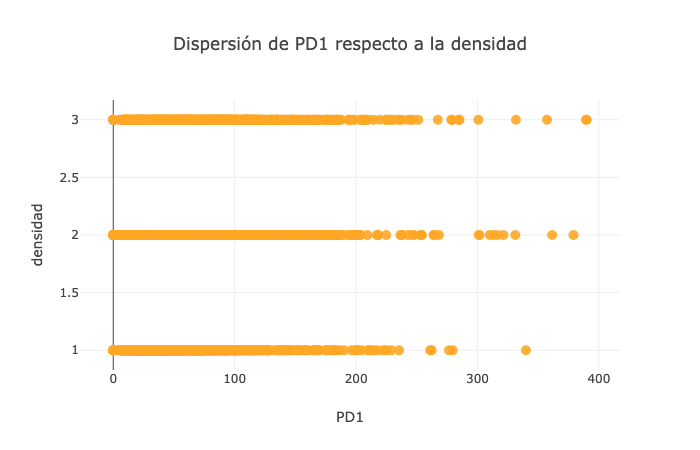
\includegraphics[scale=0.5]{d-pd1.png}
	\label{fig:dpd1}
\end{figure}

En la figura \ref{fig:dpd1} se pueden evidenciar algunos valores extremos que incluyen al valor máximo de dicha variable que es 390gr.

\begin{figure}[h!]
	\caption{Dispersión de la variable de pesos fresco del calibre 2 respecto a la densidad.}
	\centering
	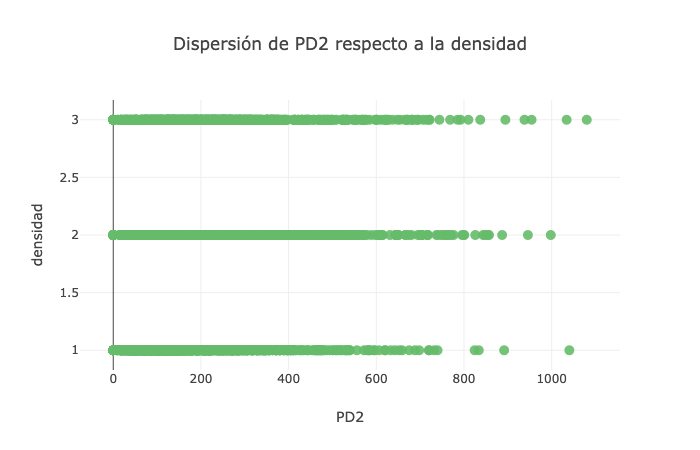
\includegraphics[scale=0.5]{d-pd2.png}
	\label{fig:dpd2}
\end{figure}

En la figura \ref{fig:dpd2} también se pueden encontrar algunos valores extremos incluyendo al valor tope de dicha variable que es 1080gr.

\begin{figure}[h!]
	\caption{Dispersión de la variable de pesos fresco del calibre 3 respecto a la densidad.}
	\centering
	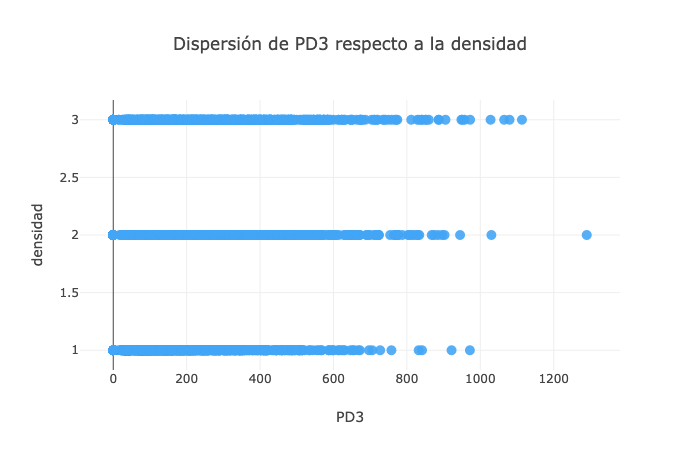
\includegraphics[scale=0.5]{d-pd3.png}
	\label{fig:dpd3}
\end{figure}

En la figura \ref{fig:dpd3} que gráfica PD3 cuyo valor máximo es 1290gr se observan varios valores extremos.

\begin{figure}[h!]
	\caption{Dispersión de la variable de pesos fresco del calibre 4 respecto a la densidad.}
	\centering
	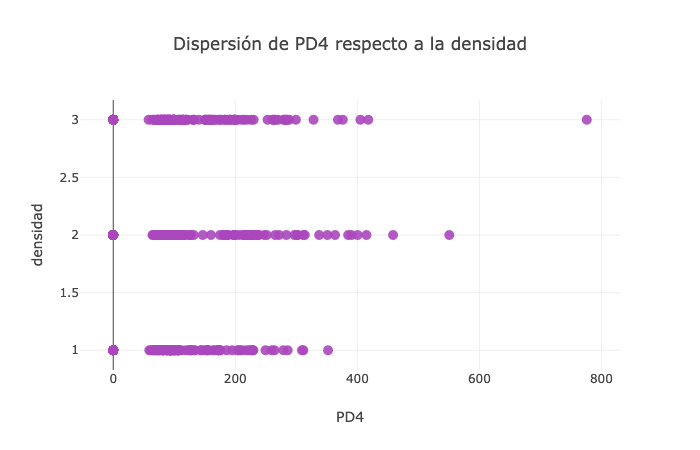
\includegraphics[scale=0.5]{d-pd4.png}
	\label{fig:dpd4}
\end{figure}

En la figura \ref{fig:dpd4} se encuentran datos con valores extremos que se encuentran muy cercanos al mínimo y máximo.

Las figuras descritas anteriormente permiten determinar que se debe realizar limpieza de datos para evitar esos valores extremos o atípicos que afectan negativamente los cálculos durante la clasificación.\\


\noindent
\textbf{Exploración de datos.}\\

Las correlaciones de las variables PD1, PD2, PD3 y PD4 para cada densidad demuestran la relación que existe entre dichas variables, en las siguientes figuras se pueden observar los valores calculados empleando el coeficiente de correlación de Spearman.\\

En las figuras \ref{fig:cd1}, \ref{fig:cd2} y \ref{fig:cd3} se observan los valores de correlación entre las variables de peso para las densidades 1, 2 y 3, los valores oscilan entre 0 y 0.6 indicando que existe una correlación positiva entre los atributos PD1, PD2, PD3 y PD4.\\\\\\\\\\\\\\\\

\begin{figure}[h!]
	\caption{Matriz de correlaciones para la densidad 1.}
	\centering
	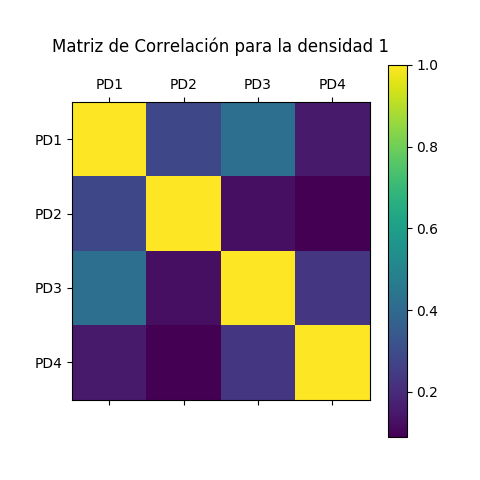
\includegraphics[scale=0.5]{correlacionD1.jpg}
	\label{fig:cd1}
\end{figure}

\begin{figure}[h!]
	\caption{Matriz de correlaciones para la densidad 2.}
	\centering
	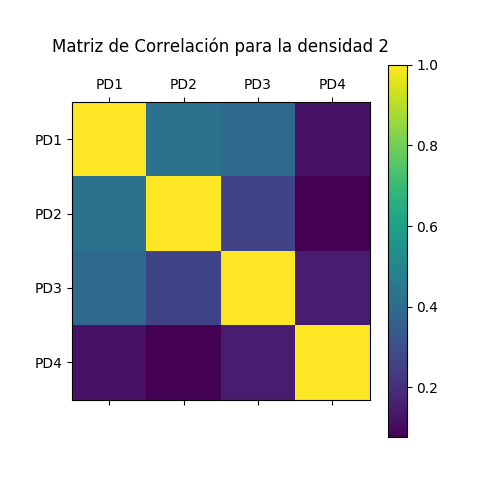
\includegraphics[scale=0.5]{correlacionD2.jpg}
	\label{fig:cd2}
\end{figure}

\begin{figure}[h!]
	\caption{Matriz de correlaciones para la densidad 3.}
	\centering
	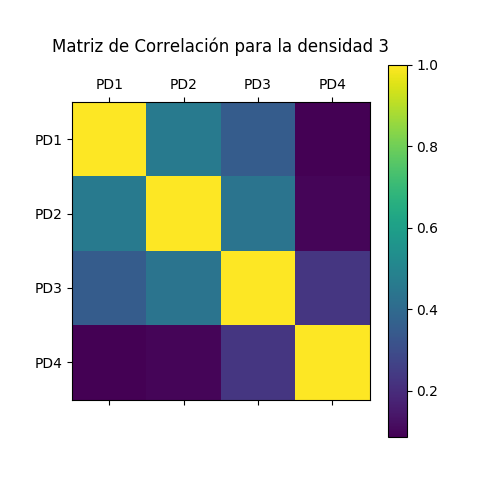
\includegraphics[scale=0.5]{correlacionD3.jpg}
	\label{fig:cd3}
\end{figure}

Tomando en cuenta los estadísticos básicos de cada conjunto de datos se logra observar que los valores de varianza para las variables PD1, PD2, PD3 y PD4 son altos, esto podría afectar negativamente los cálculos del algoritmo de clasificación. A continuación se pueden observar los
histogramas de las variables de entrada para cada densidad que permiten apreciar el patrón que siguen los datos.\\\\\\\\\\\\\\\\\\\\\\\\\\\\

\begin{figure}[h!]
	\caption{Dispersión de la variable de pesos fresco del calibre 4 respecto a la densidad.}
	\centering
	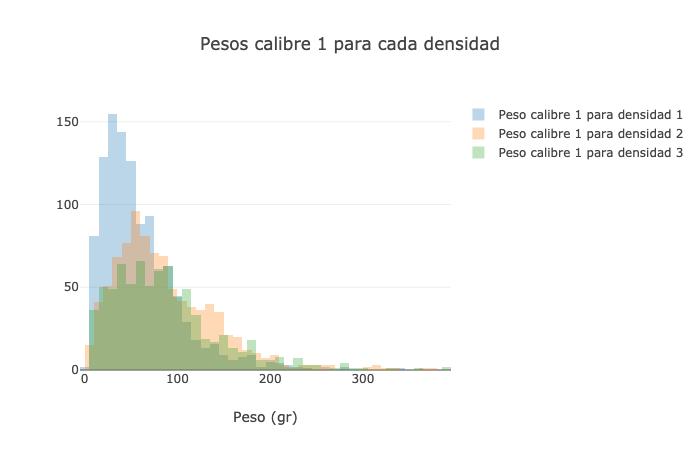
\includegraphics[scale=0.6]{PD1.png}
	\label{fig:pd1}
\end{figure}

\begin{figure}[h!]
	\caption{Dispersión de la variable de pesos fresco del calibre 4 respecto a la densidad.}
	\centering
	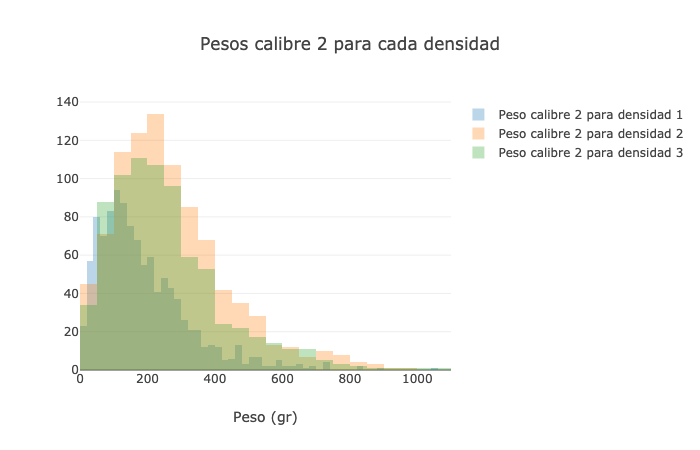
\includegraphics[scale=0.6]{PD2.png}
	\label{fig:pd2}
\end{figure}

\begin{figure}[h!]
	\caption{Dispersión de la variable de pesos fresco del calibre 4 respecto a la densidad.}
	\centering
	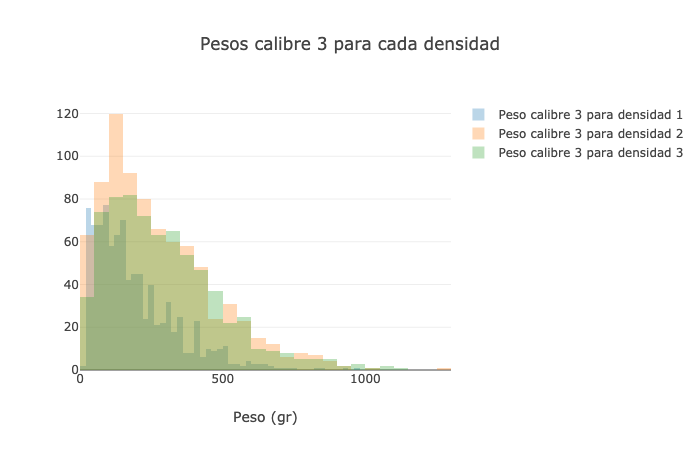
\includegraphics[scale=0.6]{PD3.png}
	\label{fig:pd3}
\end{figure}

\begin{figure}[h!]
	\caption{Dispersión de la variable de pesos fresco del calibre 4 respecto a la densidad.}
	\centering
	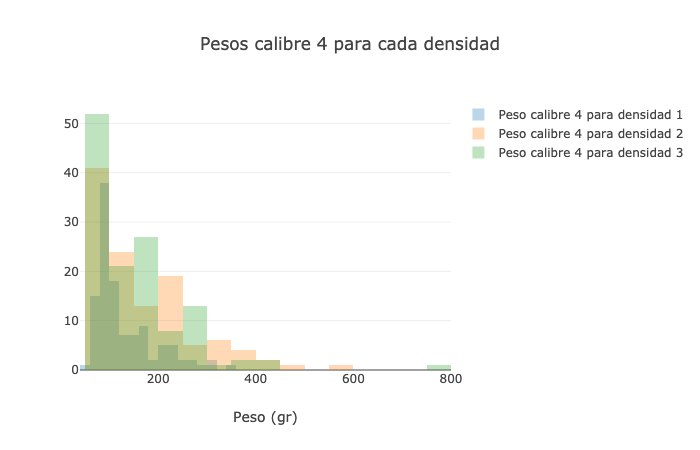
\includegraphics[scale=0.6]{PD4.png}
	\label{fig:pd4}
\end{figure}

En la figura \ref{fig:pd1} se encuentra el histograma de la variable PD1 para cada densidad, se puede ver el comportamiento de la variable demostrando diferentes patrones para cada densidad; en cuanto a la figura \ref{fig:pd2} se tiene a la variable PD2 que muestra patrones un poco mas similares para cada densidad, en la siguiente figura que es la \ref{fig:pd3} se evidencia la disminución de esta variable para la densidad 1 y finalmente en la figura \ref{fig:pd4} se hace evidente que la variable PD4 tiene valores menores respecto a las anteriores.\\

Los histogramas permiten determinar que la distribución de los datos de entrada se asemeja a una curva normal, lo que ayuda a inferir que se debe emplear el método gaussiano de Bayes Naive para realizar su clasificación.\\\\

\noindent
\textbf{Verificación de la calidad de los datos.}\\

Luego de revisar los valores de los datos se determinó que no era necesaria la estandarización de los mismos, ya que todos se encuentran en el mismo rango en cuanto a valor y en la misma unidad de peso (gramos); además no hay valores faltantes, es decir, el set de datos está completo.

\section{Preparación de datos}

\noindent
\textbf{Selección de datos.}\\

Los datos disponibles son: densidad, PD1, PD2, PD3, PD4, X y Y, sin embargo, las coordenadas de las
plantas no son un dato relevante para la clasificación que se realizó porque la misma busca determinar
la densidad sólo a partir de los pesos frescos por calibre, por lo tanto se excluyeron del set de datos.\\

Se debe tomar en cuenta que los datos de los pesos frescos por calibre fueron calculados empíricamente
lo que podría implicar tener valores erróneos.\\

\noindent
\textbf{Limpieza de los datos.}\\

No fue necesario realizar una limpieza de datos considerando la calidad de los mismos.\\

\noindent
\textbf{Estructuración de los datos.}\\

No es necesario calcular atributos derivados para realizar la clasificación; no se debe realizar
una normalización de índices porque los valores de entrada se encuentran en la misma escala y unidad, y la estimación de las varianzas indica que son homogéneos y que no existen datos atípicos o extremos.\\

\noindent
\textbf{Integración de los datos.}\\

La media y varianza son dos datos combinados calculados a partir de los datos iniciales, estos nuevos
datos son necesarios durante el cálculo probabilístico del algoritmo clasificador y se
obtienen al principio de la ejecución llamando a la función \textbf{media\_varianza} que retorna
dos arreglos matriciales \textbf{m} y \textbf{v}, con un número de filas igual a la cantidad de clases, en este caso tres filas,
y la cantidad de columnas es igual a la cantidad de características de entrada, es decir, cuatro
para la data que se está empleando, cada campo de la matriz contiene la media o varianza (dependiendo de la
matriz que se este revisando) para esa característica y esa clase.\\

\noindent
\textbf{Formato de los datos.}\\

Los datos de entrada se encuentran ordenados según su clase, por lo tanto deben ser desordenados para permitir que el algoritmo de clasificación obtenga datos de cada clase para realizar los cálculos; para desordenar las filas de datos se empleó la función \textbf{random.shuffle} del paquete \textbf{numpy} para python, para que el reordenamiento se realizada de forma aleatoria.\\

\section{Modelado}

\noindent
\textbf{Técnica de modelado.}\\

Para la clasificación de los datos se empleó un modelo probabilístico basado en el teorema de Bayes Naive para una distribución
gaussiana, se seleccionó esta técnica por tener como supuesto la independencia entre las variables y su distribución
espacial. Las pruebas del modelo se realizaron separando los datos en un set de entrenamiento que posee el 80\% de los
datos y el otro 20\% se destino al set de pruebas, luego de obtener los resultados para el set de pruebas se realiza la
evaluación del modelo empleando la curva característica operativa del receptor.\\

El desarrollo del clasificador se realizó empleando Bayes Naive Gaussiano como se indica anteriormente, luego de leer los datos se llama a la función
\textbf{bayes\_naive\_gaussiano} que recibe como entrada los siguientes parámetros:
\begin{itemize}
	\item{set\_entrenamiento: es un array de numpy con las columnas número de planta, densidad, PD1, PD2, PD3, PD4, X y Y, su
	cantidad de filas depende de la cantidad de datos que sean destinados a formar parte del entrenamiento que en este caso es
	el 80\% de los datos iniciales, es decir, aproximadamente 2272 filas.}
	\item{set\_test: es un array de numpy con las columnas PD1, PD2, PD3 y PD4, su cantidad de filas depende de la cantidad de
	datos que sean destinados a formar parte del set de pruebas que en este caso es el 20\% de los datos iniciales, es decir,
	aproximadamente 567 filas.}
	\item{clases\_set\_test: es un array de numpy y cada fila representa la clase (densidad) para los datos en el set de test
	en el mismo número de fila, su cantidad de filas depende de la cantidad de datos que sean destinados a formar parte del set
	de pruebas que en este caso es el 20\% de los datos iniciales, es decir, aproximadamente 567 filas.}
\end{itemize}

Luego se ejecutan los siguientes pasos:
\begin{enumerate}
	\item Cálculo de la media y varianza:
	como se indicó previamente los valores de las medias y varianzas de cada característica para cada clase son necesarios
	para realizar los cálculos probabilísticos, en este paso del algoritmo se llama a la función \textbf{media\_varianza}, para
	realizar dicho procedimiento empleando para la media la fórmula: \[\bar{x}=\frac{\sum_{i=1}^n{x_{i}}}{n}\] y para la varianza:
	\[\sigma^2=\frac{\sum_{i=1}^n{\left(x_{i}-\bar{x}\right)^2}}{n - 1}\]\\
	\item Cálculo de probabilidades previas:
	ejecuta la función \textbf{pre\_prob} que recibe un vector unidimensional con los valores de las clases
	del set de entrenamiento y aplica la fórmula
	\[Prob\;Previa\left(c\right)=\frac{ocurrencias\;de\;la\;clase\;c}{Nro\;total\;de\;datos}\]
	retornando un vector unidimensional con la probabilidad previa de cada clase.\\
	\item Cálculo de la probabilidad posterior:
	es necesario calcular la probabilidad posterior del set de pruebas dada una clase \textbf{c},
	para ello se llama al método \textbf{prob\_caracteristica\_clase} que recibe como
	parámetros la matriz de medias, la matriz de varianzas y el set de pruebas; tomando en cuenta la
	fórmula para el cálculo de probabilidades de una distribución gaussiana:
	\[
	P\left(x\right) = \frac{1}{\sqrt{2\pi\sigma^{2}}}e^{-\frac{\left(x-\mu\right)^{2}}{2\sigma^{2}}}
	\]
	se puede definir que la probabilidad posterior para una característica del set de prueba dada una
	clase \textbf{c} es:
	\[
	P\left(x_{i}|c\right) = \frac{1}{\sqrt{2\pi\sigma^{2}_{x_{i},c}}}
	e^{-\frac{\left(x_{i}-\bar{x}_{x_{i},c}\right)^{2}}{2\sigma^{2}_{x_{i,c}}}}
	\]
	donde $x_{i}$ es una característica de esa fila del set de datos; el código de la función se encarga de
	obtener el resultado de esa fórmula para cada característica dentro de la fila del set de datos para
	la clase dada y luego multiplica los valores de dichas probabilidades obteniendo la probabilidad posterior
	para esa clase. Esta función retorna una matriz con una cantidad de filas igual a las filas del set de
	pruebas y por cada fila posee varios valores, cada uno de estos indica la probabilidad posterior para una clase.\\

	\item Obtiene las probabilidades condicionales y las predicciones:
	finalmente para calcular la probabilidad condicional de una instancia de test se emplea la función
	\textbf{prob\_condicional} que recibe como parámetros el set de pruebas, la cantidad de clases, el
	arreglo con las probabilidades posteriores, el arreglo con las probabilidades previas y las verdaderas
	clases del set de pruebas; empleando el teorema de Bayes obtiene la probabilidad condicional de cada
	clase para una fila del set de pruebas:
	\[P\left(c_{i}|x\right)=
	\frac{P\left(c_{i}\right)P\left(x|c_{i}\right)}{\sum_{j=1}^{n}P\left(c_{j}\right)P\left(x|c_{j}\right)}
	\]
	Luego se toma la probabilidad condicional mayor entre las calculadas para ese set de prueba
	obteniendo así la predicción.
\end{enumerate}

\noindent
\textbf{Método de evaluación de los modelos.}\\

Para evaluar el modelo se emplean curvas ROC, primero se realiza el cálculo de la matriz de confusión empleando la función
\textbf{confusion\_matrix} del módulo \textbf{metrics} del paquete \textbf{sklearn}
y posteriormente se realiza la curva característica operativa del receptor con el enfoque multiclase usando los métodos
\textbf{roc\_curve} y \textbf{auc} del mismo paquete, el primer método computa la curva ROC graficando las fracciones de
verdaderos positivos y falsos positivos para distintos umbrales, y la función \textbf{auc} computa el área bajo la curva.
Según Ato y López (1995) un área bajo la curva igual a 1 correspondería a una prueba diagnóstica perfecta y un
área bajo la curva igual a 0.5 indica que se obtuvo una prueba sin precisión diagnóstica.

\section{Evaluación}

\noindent
\textbf{Evaluación de los resultados.}\\

Cada vez que se ejecuta el algoritmo el mismo indica que obtuvo un porcentaje de aciertos de aproximadamente
45\% y de desaciertos de aproximadamente 55\%, en cada corrida los datos que emplea el algoritmo para entrenamiento
y prueba varían por lo tanto estos valores pueden cambiar ligeramente. En cuanto a la curva característica
operativa del receptor se obtiene:


\begin{figure}[h!]
	\caption{Matriz de correlaciones para la densidad 3.}
	\centering
	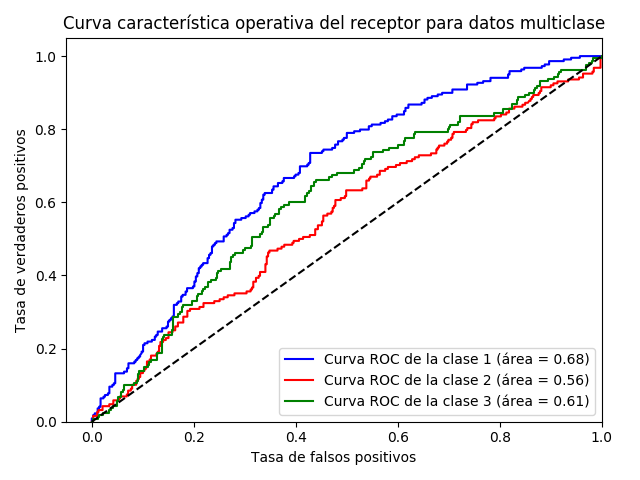
\includegraphics[scale=0.55]{roc.png}
	\label{fig:roc}
\end{figure}

La curva ROC en la figura \ref{fig:roc} posee trazos que indican que no es una mala clasificación pero tampoco es una clasificación
óptima, si se observan los valores para el área bajo la curva de la densidad 1, 2 y 3
se obtuvieron 0.68, 0.56 y 0.61 respectivamente que según el estándar indicado anteriormente
están entre una precisión regular y no tener precisión diagnóstica.\\

Se puede demostrar que el algoritmo está generando una clasificación empleando el método de Bayes Naive Gaussiano
y está obteniendo los resultados del método de evaluación, aunque los mismos no sean los deseados.\\

\noindent
\textbf{Proceso de revisión.}\\

Los objetivos de este proceso fueron diagnósticar el formato de las
variables de entrada y salida para el clasificador, establecer el tipo de
algoritmo de Bayes Naive a emplear y las características para el entrenamiento,
realizar la implementación del algoritmo, realizar las pruebas de funcionamiento
y la comparación estadística, todos estos objetivos fueron cubiertos durante el
desarrollo de esta metodología y se logró el diseño de un clasificador de tubérculos
de papa criolla para diferentes densidades de siembra a partir de los pesos frescos
por calibre empleando Bayes Naive.\\

\noindent
\textbf{Determinación de futuras fases.}\\

En cuanto al proceso actual algunas mejoras posibles podrían ser la eliminación
de las características con valores iguales a cero o emplear otros métodos para
clasificar los datos como las redes neuronales, se podría implementar un análisis
espacial e incluso realizar una revisión más profunda a los datos, cualquiera de
estás alternativas podría mejorar o empeorar el porcentaje de aciertos de la clasificación actual.\\

Según Rish (2001) existen características dentro de los datos que pueden afectar el
rendimiento de Bayes Naive, como el impacto generado por la entropía de la distribución, la
cantidad de información despreciada por asumir la independencia de las entradas, entre otros,
sería bueno identificar estas características dentro del set de datos empleados para la prueba de
este clasificador y así lograr determinar que está afectando la clasificación.